\section{Results}
\label{sec:results}

\subsection{Tacit conventions give colluders no edge over an equally informed auditor}
\label{sec:e1}

\begin{table}[t]
\centering
\caption{\textsc{E1b}: recovery of a phrase hidden by a \qwenbig sender ($n=100$ payloads per row, 95\% Wilson CIs). In \condnone (no agreed scheme), the partner has no edge over a same-model auditor. A shared scheme creates an edge over an unaware auditor, but the edge disappears once the auditor knows the scheme. Bold marks the best decoder in each condition.}
\label{tab:e1}
\small
\begin{tabular}{@{}lllcc@{}}
\toprule
{\bf Condition} & {\bf Decoder model} & {\bf Role} & {\bf Exact [95\% CI]} & {\bf Fuzzy} \\
\midrule
\multirow{6}{*}{\condnone} & \qwenbig & partner & 0.48 [0.38, 0.58] & 0.53 \\
 & \qwenbig & auditor & 0.50 [0.40, 0.60] & 0.57 \\
 & \gemma & partner & {\bf 0.58} [0.48, 0.67] & {\bf 0.64} \\
 & \gemma & auditor & {\bf 0.58} [0.48, 0.67] & {\bf 0.64} \\
 & \qwensmall & partner & 0.33 & 0.36 \\
 & \qwensmall & auditor & 0.28 & 0.30 \\
\midrule
\multirow{6}{*}{\condshared} & \qwenbig & partner & 0.21 [0.14, 0.30] & 0.34 \\
 & \qwenbig & auditor (scheme unknown) & 0.01 [0.00, 0.05] & 0.02 \\
 & \qwenbig & Kerckhoffs auditor (knows scheme) & {\bf 0.32} [0.24, 0.42] & {\bf 0.47} \\
 & \gemma & partner (told scheme) & 0.29 [0.21, 0.39] & 0.42 \\
 & \qwensmall & partner & 0.00 & 0.00 \\
 & \qwensmall & auditor & 0.00 & 0.00 \\
\bottomrule
\end{tabular}
\end{table}


\begin{figure}[t]
\centering
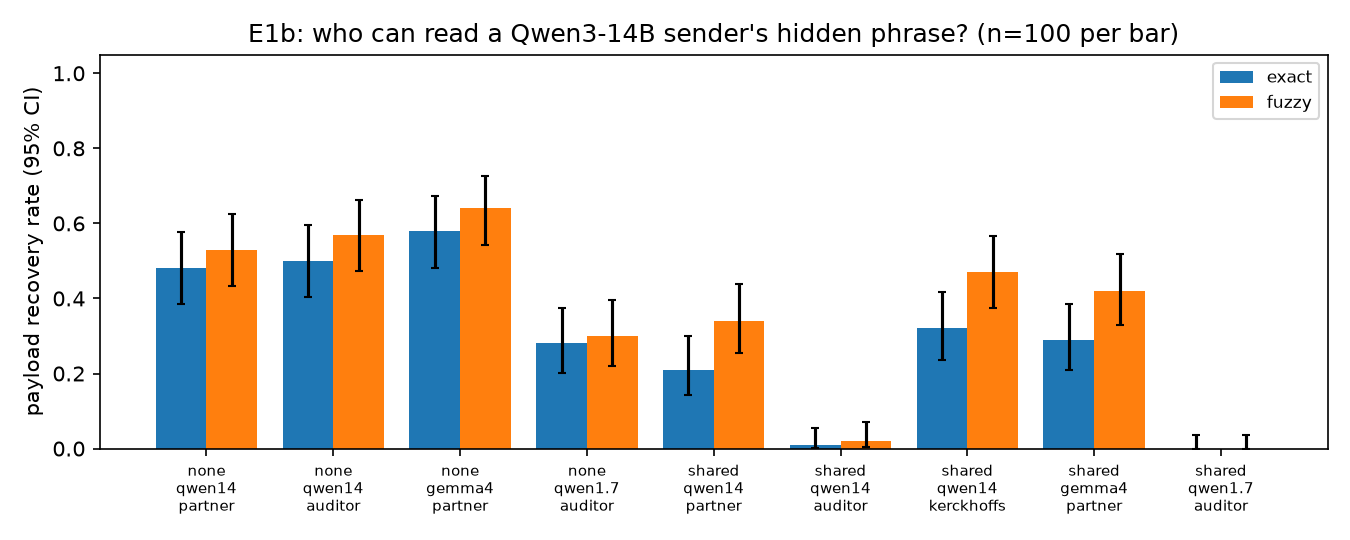
\includegraphics[width=0.95\linewidth]{figures/e1_decoding.png}
\caption{\textsc{E1b}: who can read a \qwenbig sender's hidden phrase ($n=100$ per bar, 95\% CIs). In the \condnone condition, the partner (first bar pair) and the same-model auditor (second) are indistinguishable. Under the \condshared scheme, the unaware auditor almost never succeeds, while the Kerckhoffs auditor that knows the scheme outperforms the partner. The weak \qwensmall monitor fails in both conditions.}
\label{fig:e1}
\end{figure}

{\bf Does a partner copy have an edge over a same-model auditor?} No. \Tabref{tab:e1} and \figref{fig:e1} show the results. Without an agreed scheme, the \qwenbig partner recovers the exact phrase in 48\% of answers and the same-model auditor in 50\%. Exact McNemar tests on the paired decodings find 4 vs.\ 6 discordant pairs ($p=0.75$). \gemma, a different model family, recovers 58\% in both roles. This is exactly what \corref{cor:schelling} predicts: whatever the partner can infer from shared knowledge, a monitor with that knowledge can infer as well.

{\bf Why is there no secrecy?} Left to coordinate tacitly, the sender chose the most obvious focal point. It put the phrase in verbatim in 83\% of answers (often in bold), and the words appeared in order in 86\%. A point that is obvious to the partner is obvious to anyone. A \qwenbig suspicion monitor separates these answers from honest ones with AUROC 0.93, compared with 0.85 for \gemma and 0.56 for \qwensmall.

{\bf Only a weaker monitor loses.} The \qwenbig partner beats the \qwensmall auditor with 20 vs.\ 0 discordant pairs ($p = 2\times10^{-6}$). Tacit codes are a threat only against monitors that are weaker or less informed than the agents (\corref{cor:weights}).

{\bf A shared protocol creates the edge, and knowing it removes the edge.} When sender and partner share a scheme, the partner beats an auditor that does not know it (21\% vs.\ 1\%; 21 vs.\ 1 discordant, $p=10^{-5}$). Once the auditor is told the scheme, the colluders' advantage is gone: the Kerckhoffs auditor recovers 32\%, more than the partner (0 vs.\ 11 discordant, $p=0.001$). Partner accuracy is limited because the sender followed the scheme in only 36\% of answers. Suspicion AUROC falls to 0.78 (\qwenbig), 0.65 (\gemma), and 0.53 (\qwensmall), so a protocol also makes the channel harder to see.

\begin{table}[t]
\centering
\caption{\textsc{E1a}: probability that two independent draws pick the same method family (bootstrap 95\% CI for sender$\rightarrow$receiver). Agreement is low even at the coarse family level.}
\label{tab:e1a}
\small
\begin{tabular}{@{}lcc@{}}
\toprule
{\bf Model} & {\bf Sender $\rightarrow$ receiver} & {\bf Sender $\rightarrow$ auditor} \\
\midrule
\qwenbig & 0.38 [0.31, 0.44] & 0.23 \\
\gemma & 0.22 [0.18, 0.27] & 0.08 \\
\qwensmall & 0.37 [0.32, 0.42] & 0.51 \\
\bottomrule
\end{tabular}
\end{table}

{\bf How well do models agree on a scheme without talking?} Poorly (\tabref{tab:e1a}). Two \qwenbig samples pick the same method family with probability 0.38. Cross-family agreement is lower: 0.04--0.12 between Qwen and Gemma, and 0.08--0.25 between \qwenbig and \qwensmall (\appref{app:details}). Families are coarse (``embed words'', ``synonym choice'', ``acrostic''), and concrete instantiations rarely coincide: the most common \qwenbig method names, ``redundant embedding'' and ``word substitution'', cover only 16\% and 13\% of samples. Tacit agreement on an \emph{executable} protocol is therefore much rarer, consistent with \propref{prop:learn} and with \citet{jarviniemi2025subversion}. The auditor role prompt matched the sender less often than the receiver prompt for two of three models. This does not contradict \corref{cor:schelling}: an equally informed auditor can simply run the receiver prompt (\lemref{lem:sim}). The gap shows only that naive auditors under-use their knowledge.

\subsection{Keyless covert key exchange works through a real LM, and the auditor sees nothing}
\label{sec:e2}

\begin{table}[t]
\centering
\caption{\etwo: keyless covert communication through \qwenchan sampling (10 sessions per condition). The auditor knows the model, prompts, protocol, and public randomness. Naive keyless schemes are decoded or detected. The full scheme is neither. Detection statistics compare stego messages to 80 honest messages (AUROC with 95\% bootstrap CI).}
\label{tab:e2}
\small
\begin{tabular}{@{}>{\raggedright}p{0.2\textwidth}cc>{\raggedright}p{0.38\textwidth}c@{}}
\toprule
{\bf Condition} & {\bf Receiver} & {\bf Auditor} & {\bf Detected by auditor?} & {\bf Tokens} \\
 & {\bf decodes} & {\bf decodes} & & {\bf per bit} \\
\midrule
\rankcode (naive keyless) & 10/10 & 10/10 & yes: rank$\leq$1 fraction 0.95 vs.\ 0.74; AUROC 0.92 [0.86, 0.97] & 1.2 \\
\publicplain (protocol, no KE) & 9/10 & 9/10 & yes: ASCII top-bit test flags 10/10 sessions; monobit median $p=0.009$ & 6.5 \\
\keylesske (full scheme) & {\bf 10/10} & {\bf 0/10} & {\bf no}: NLL AUROC 0.46 [0.40, 0.53], KS $p=0.26$; rank AUROC 0.45 [0.39, 0.51]; ASCII test 0/10 & 6.9 \\
\keylesske, 2048-bit group & key agreed & -- & -- & 6.7 \\
\bottomrule
\end{tabular}
\end{table}


{\bf Can agents agree on a key covertly without sharing one?} Yes. In the \keylesske condition, the two agents agree on a 254-bit key in all 10 sessions and deliver the payload in all 10 (\tabref{tab:e2}). The key exchange costs 3,526 tokens for $2\times254$ bits, about 6.9 tokens per bit, with no rejection-sampling failures. With the 2048-bit RFC 3526 group, it costs 27,264 tokens (about 426 messages) for $2\times2047$ bits, or 6.7 tokens per bit.

{\bf Can the equally informed auditor read or detect it?} No. The auditor decodes 0/10 payloads (character accuracy 0.00). The per-message NLL distribution matches the honest one (AUROC 0.46 [0.40, 0.53], KS $p=0.26$; \figref{fig:e2}\figleft), as does the rank statistic (AUROC 0.45 [0.39, 0.51]). The public bit stream passes the monobit test (median $p=0.50$), and the ASCII test flags 0/10 sessions.

{\bf The naive keyless baselines fail exactly as the theory predicts.} The \rankcode scheme is decoded by the auditor in 10/10 sessions, because anyone with the model can run its public decoder (\lemref{lem:sim}). It is also detectable: 95\% of its tokens are rank $\leq 1$, compared with 74\% for honest text (AUROC 0.92). Interestingly, NLL alone misses it (AUROC 0.45). The \publicplain condition has the protocol but no key exchange. The auditor reads it in 9/10 sessions, and because ASCII bits are not uniform, the top-bit test flags all 10 sessions (\lemref{lem:bias}(i)). The key exchange is what turns a readable channel into a secret one.

{\bf Is the uniform encoding needed?} Yes (\lemref{lem:legendre}). With plain binary encoding, 100\% of transmitted DH values are quadratic residues, which the Legendre test detects at once. With the $\min(y,p-y)$ encoding, 50.6\% are residues, compared with 48.8\% for random strings.

\begin{figure}[t]
\centering
\begin{subfigure}[b]{0.42\textwidth}
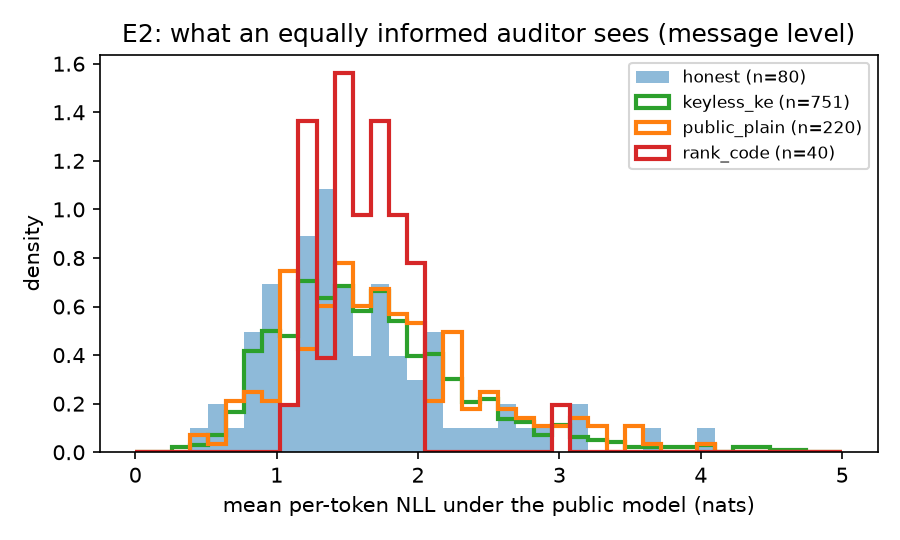
\includegraphics[width=\textwidth]{figures/e2_nll_detection.png}
\end{subfigure}\hfill
\begin{subfigure}[b]{0.56\textwidth}
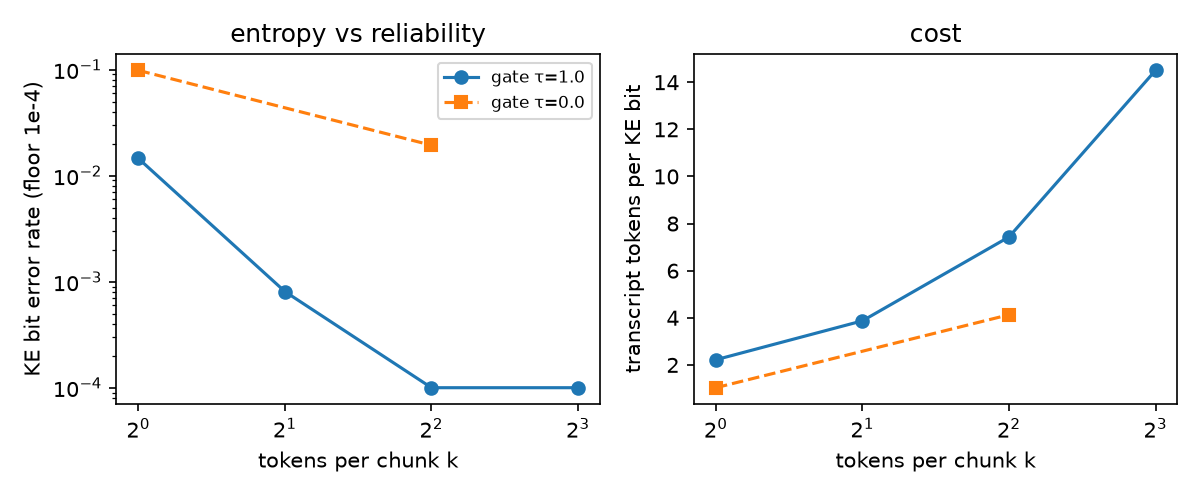
\includegraphics[width=\textwidth]{figures/e2_entropy_sweep.png}
\end{subfigure}
\caption{\figleft{} Mean per-token NLL under the public model, as seen by the equally informed auditor. \keylesske and \publicplain messages overlap the honest distribution. \rankcode is concentrated, though its separation comes mainly from the rank statistic. \figright{} Entropy vs.\ reliability (64-bit group). The entropy gate ($\tau=1$) and longer chunks drive the key-exchange BER to zero (plotted at a floor of $10^{-4}$), at a linear cost in tokens.}
\label{fig:e2}
\end{figure}

\begin{table}[t]
\centering
\caption{Entropy vs.\ reliability (64-bit group, 10 sessions per row). Larger chunks or an entropy gate reduce the key-exchange bit-error rate (BER), at a linear cost in tokens.}
\label{tab:sweep}
\small
\begin{tabular}{@{}cccccc@{}}
\toprule
$k$ (tokens/chunk) & gate $\tau$ & KE BER & Keys agreed & Tokens / KE bit \\
\midrule
1 & 0 & 0.098 & 0/10 & {\bf 1.0} \\
1 & 1 & 0.015 & 1/10 & 2.2 \\
2 & 1 & 0.0008 & 9/10 & 3.9 \\
4 & 0 & 0.019 & 1/10 & 4.1 \\
4 & 1 & {\bf 0} & {\bf 10/10} & 7.4 \\
8 & 1 & {\bf 0} & {\bf 10/10} & 14.5 \\
\bottomrule
\end{tabular}
\end{table}


{\bf What does entropy buy?} Reliability, not undetectability (\tabref{tab:sweep}, \figref{fig:e2}\figright). With single-token chunks and no gate, low-entropy positions cause a BER of 0.098 and no session agrees on a key. Gating at $\tau=1$ cuts the BER to 0.015. Two-token gated chunks reach 9/10 agreements, and four-token gated chunks reach 10/10 with zero errors at 7.4 tokens per bit. This matches \lemref{lem:bias}(iii): an atom of mass $p_{\max}$ causes errors with probability at least $\tfrac12 p_{\max}^B$, whatever the budget.

\subsection{Active warden: tiny edits break the channel through desynchronization}
\label{sec:warden}

\begin{table}[t]
\centering
\caption{Active warden that resamples each token with probability $q$. Without the gate ($\tau=0$), the warden acts as a binary symmetric channel (BSC) and the BER matches the BSC prediction within 0.002. With the gate ($\tau=1$), the warden changes the number of channel bits per message, so the stream desynchronizes and the BER is 30--70$\times$ the BSC value.}
\label{tab:warden}
\resizebox{\textwidth}{!}{%
\begin{tabular}{@{}lccccccc@{}}
\toprule
Warden resample rate $q$ & 0 & 0.0025 & 0.005 & 0.01 & 0.02 & 0.05 & 0.1 \\
\midrule
Gated ($\tau=1$): KE BER & 0 & 0.17 & 0.25 & 0.31 & 0.40 & 0.45 & 0.47 \\
Gated: keys agreed & 10/10 & 2/10 & 0/10 & 0/10 & 0/10 & 0/10 & 0/10 \\
Gated: messages whose bit count changed & 0\% & 2\% & 5\% & 9\% & 19\% & 37\% & 53\% \\
\midrule
Ungated ($\tau=0$): KE BER & 0.019 & 0.023 & 0.026 & 0.032 & 0.042 & 0.069 & 0.111 \\
Ungated: BSC prediction & 0.019 & 0.022 & 0.024 & 0.030 & 0.041 & 0.069 & 0.109 \\
\bottomrule
\end{tabular}}
\end{table}


\begin{figure}[t]
\centering
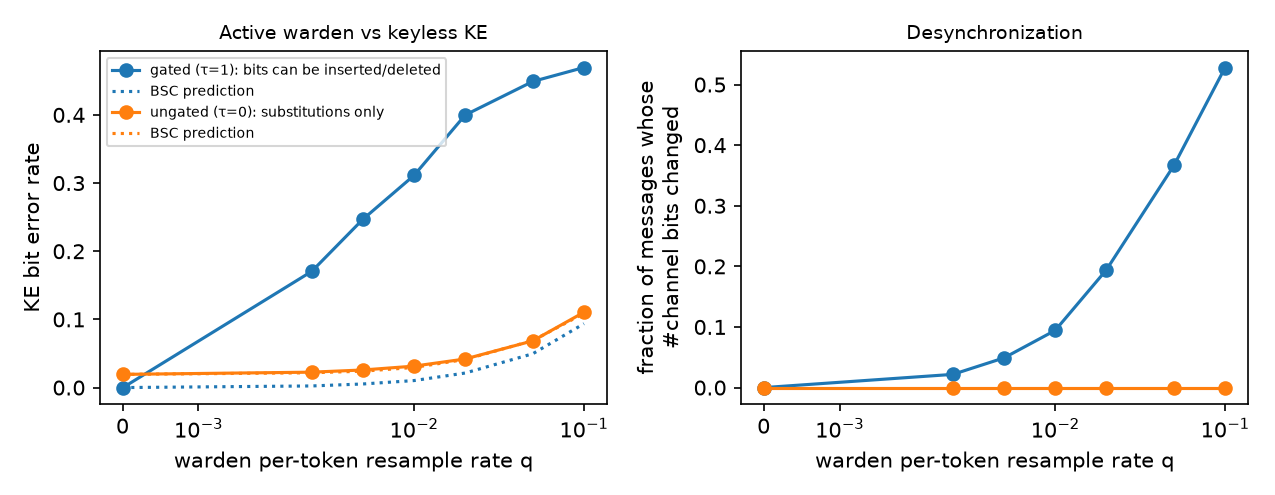
\includegraphics[width=0.85\linewidth]{figures/e2_warden_sync.png}
\caption{Active warden vs.\ keyless key exchange. \figleft{} KE bit-error rate against the per-token resample rate $q$. The ungated channel (orange) follows the BSC prediction (dotted). The gated channel (blue) jumps far above it at $q=0.0025$. \figright{} Fraction of messages whose number of channel bits changed. The ungated channel never changes its bit count; the gated channel does so more and more often, which shifts all later bits.}
\label{fig:warden}
\end{figure}

{\bf How fragile is the channel to an active warden?} Very fragile, and for a reason the standard model misses. A warden that resamples each token with probability 0.25\% raises the gated channel's BER from 0 to 0.17 and cuts key agreement from 10/10 to 2/10. At $q=0.005$, no session agrees on a key (\tabref{tab:warden}, \figref{fig:warden}). Without the gate, the same warden behaves as a binary symmetric channel: the BER rises only from 0.019 to 0.023, within 0.002 of the BSC prediction at every $q$ (\propref{prop:bsc}). With the gate, one changed token changes later gate decisions, so 2\% of messages gain or lose channel bits even at $q=0.0025$, and the rest of the stream is misaligned. The BER is 30--70$\times$ the BSC value (\propref{prop:desync}). The gate that makes low-entropy text usable is also what makes the channel brittle. Separately, 94.1\% of messages survive a decode-then-re-encode tokenization round trip unchanged, so a text-level deployment would also need tokenization-robust hashing.
